\documentclass[../../dissertation.tex]{subfiles}
\begin{document}

The process for defining the search problem in this model is similar to the coined quantum walk case. The oracle still inverts the sign of a certain state and amplifies it, and the system's state will still be described by equation \ref{eq:sysStateSearch}. However,instead of using a coin, the staggered model takes advantage of the notions of cliques and tessellations, as was shown in chapter \ref{stagWalk}, which means the unmodified evolution operator has to be defined for an undirected complete graph.\par
As was shown in figure \ref{fig:undCompGraph}, the vertices in a complete graph are all neighbors. This is a special case because this is the only connected graph where the tessellation cover can be done by one tessellation, since the graph is it's own clique. The minimum tessellations required to cover this structures are defined by the one clique that encompasses all $N$ nodes of the graph
\begin{equation}
	\mathscr{T}_{\alpha} = \{\{0,1,2,...,N-1\}\}.
\end{equation}\par
The associated polygon can then be described as the balanced superposition of all the nodes in the graph
\begin{equation}
	\ket{\alpha} = \frac{1}{\sqrt{N}} \sum_{v=0}^{N-1} \ket{v}.
\end{equation}\par
The Hamiltonian, as defined in \ref{eq:StagHamil}, is 
%TODO: \textcolor{red}{falta índice no somatório}
\begin{equation}
	H_\alpha = 2\sum_0^1\ket{\alpha}\bra{\alpha} - I = 2\ket{\alpha_0}\bra{\alpha_0} - I
\end{equation}\par
The unmodified evolution operator from equation \ref{eq:stagWalkUnmodOp}
\begin{equation}
	U = e^{i\theta_{k}H_{k}}...e^{i\theta_{2}H_{2}}e^{i\theta_{1}H_{1}}
\end{equation}
reduces to the single Hamiltonian case
\begin{equation}
	U = e^{i\theta H_\alpha}.
	\label{eq:stagQWSearchUnmodEvo1}
\end{equation}\par
The choice of the $\theta$ value is an important one, since maximum probability is achieved at $\theta = \frac{\pi}{2}$, as shown in figure \ref{fig:stagMultTheta}.
\begin{figure}[!h]
	\centering
	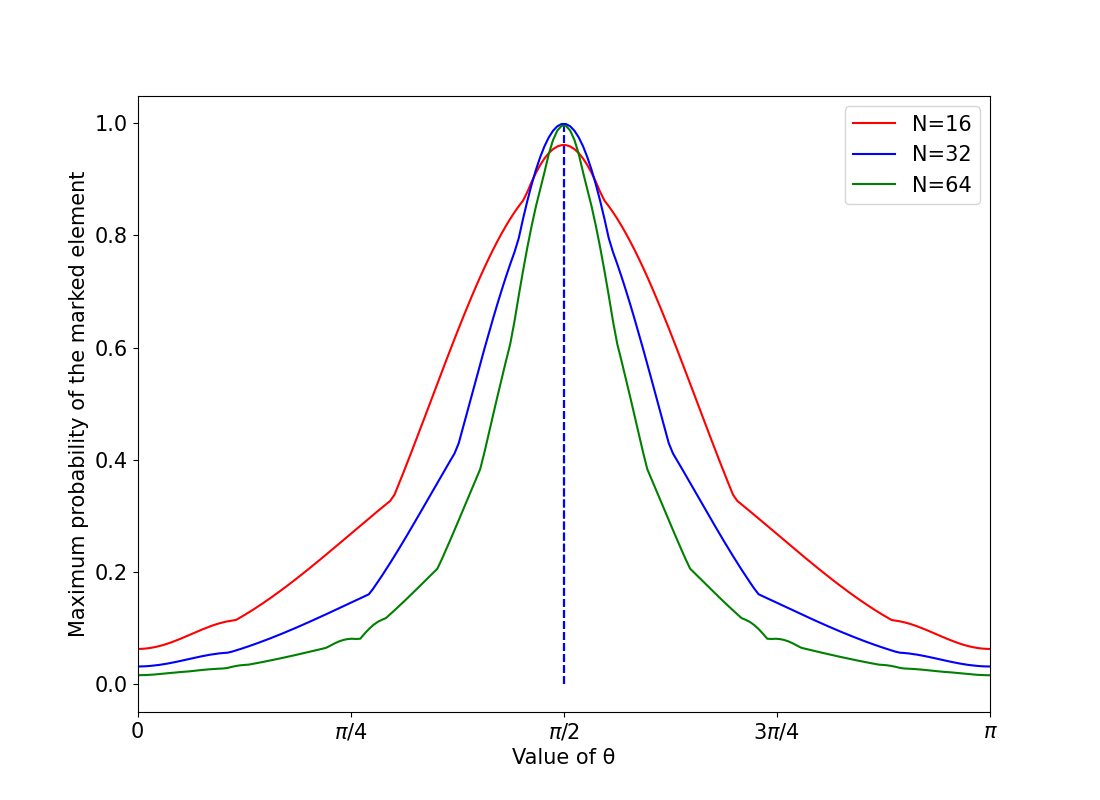
\includegraphics[scale=0.40]{img/StagQuantumWalk/Search/Theta163264.png}
	\caption{Maximum probability of the marked element as a function of the $\theta$ value plotted from $0$ to $\pi$ for number of nodes $N=64,128$ and $256$.} 
	\label{fig:stagMultTheta}
\end{figure}
Since $H_\alpha^2 = I$, equation \ref{eq:stagQWSearchUnmodEvo1} can be rewritten as
\begin{equation}
	U = e^{-i\frac{\pi}{2} H_\alpha} = \cos{\frac{\pi}{2}I} + i\sin{\frac{\pi}{2}H_\alpha} = i H_\alpha = i(2\ket{\alpha_0}\bra{\alpha_0} - I).
\end{equation}\par
Having defined the the evolution operator associated with the complete graph, the next step is to use the oracle
\begin{equation}
	\mathcal{O} = I_N - 2\ket{0}\bra{0},
\end{equation}
to create the modified evolution operator associated with the search
\begin{equation}
	U' = U\mathcal{O}.
	\label{eq:stagSearchSimulModEvoOp}
\end{equation}\par
The walk achieves the same result as Grover's algorithm after $\frac{\pi}{4}\sqrt{N}$ steps, as shown in figure \ref{fig:StagSearch}. This plot also shows that the probabilities converge to $1$ as $N$ increases, this is because time is discretized and deviations to the ideal steps will matter less for bigger values of $N$.
\begin{figure}[!h]
	\centering
	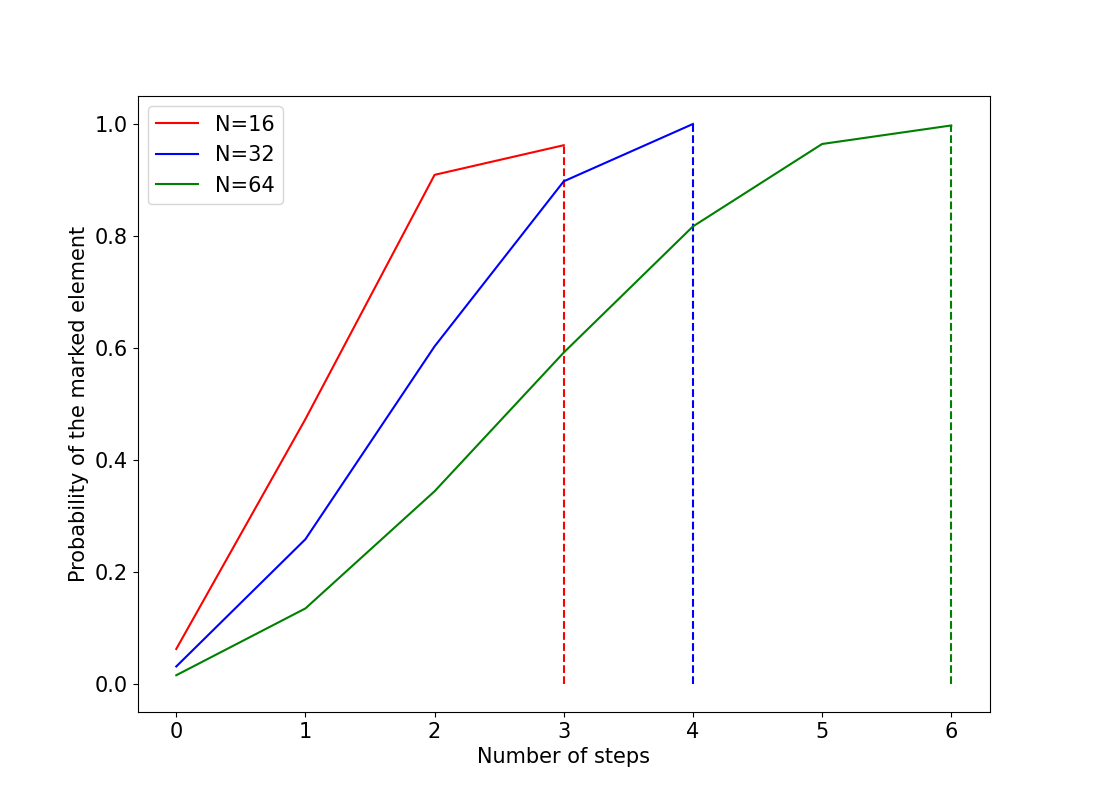
\includegraphics[scale=0.40]{img/StagQuantumWalk/Search/163264.png}
	\caption{Staggered quantum walk search for a complete graph with 16, 32 and 64 nodes.}
	\label{fig:StagSearch}
\end{figure}

%probabilidade em pi/4 sqrt(N)
%probabilidade mais perto de 1 quanto maior o N, devido à natureza discreta da walk.

%TODO:\textcolor{red}{precisa de um fechamento também aqui}


\end{document}
